\documentclass[11pt,preprint, authoryear]{elsarticle}

\usepackage{lmodern}
%%%% My spacing
\usepackage{setspace}
\setstretch{1.2}
\DeclareMathSizes{12}{14}{10}{10}

% Wrap around which gives all figures included the [H] command, or places it "here". This can be tedious to code in Rmarkdown.
\usepackage{float}
\let\origfigure\figure
\let\endorigfigure\endfigure
\renewenvironment{figure}[1][2] {
    \expandafter\origfigure\expandafter[H]
} {
    \endorigfigure
}

\let\origtable\table
\let\endorigtable\endtable
\renewenvironment{table}[1][2] {
    \expandafter\origtable\expandafter[H]
} {
    \endorigtable
}


\usepackage{ifxetex,ifluatex}
\usepackage{fixltx2e} % provides \textsubscript
\ifnum 0\ifxetex 1\fi\ifluatex 1\fi=0 % if pdftex
  \usepackage[T1]{fontenc}
  \usepackage[utf8]{inputenc}
\else % if luatex or xelatex
  \ifxetex
    \usepackage{mathspec}
    \usepackage{xltxtra,xunicode}
  \else
    \usepackage{fontspec}
  \fi
  \defaultfontfeatures{Mapping=tex-text,Scale=MatchLowercase}
  \newcommand{\euro}{€}
\fi

\usepackage{amssymb, amsmath, amsthm, amsfonts}

\def\bibsection{\section*{References}} %%% Make "References" appear before bibliography


\usepackage[round]{natbib}

\usepackage{longtable}
\usepackage[margin=2.3cm,bottom=2cm,top=2.5cm, includefoot]{geometry}
\usepackage{fancyhdr}
\usepackage[bottom, hang, flushmargin]{footmisc}
\usepackage{graphicx}
\numberwithin{equation}{section}
\numberwithin{figure}{section}
\numberwithin{table}{section}
\setlength{\parindent}{0cm}
\setlength{\parskip}{1.3ex plus 0.5ex minus 0.3ex}
\usepackage{textcomp}
\renewcommand{\headrulewidth}{0.2pt}
\renewcommand{\footrulewidth}{0.3pt}

\usepackage{array}
\newcolumntype{x}[1]{>{\centering\arraybackslash\hspace{0pt}}p{#1}}

%%%%  Remove the "preprint submitted to" part. Don't worry about this either, it just looks better without it:
\journal{Journal of Finance}

 \def\tightlist{} % This allows for subbullets!

\usepackage{hyperref}
\hypersetup{breaklinks=true,
            bookmarks=true,
            colorlinks=true,
            citecolor=blue,
            urlcolor=blue,
            linkcolor=blue,
            pdfborder={0 0 0}}


% The following packages allow huxtable to work:
\usepackage{siunitx}
\usepackage{multirow}
\usepackage{hhline}
\usepackage{calc}
\usepackage{tabularx}
\usepackage{booktabs}
\usepackage{caption}


\newenvironment{columns}[1][]{}{}

\newenvironment{column}[1]{\begin{minipage}{#1}\ignorespaces}{%
\end{minipage}
\ifhmode\unskip\fi
\aftergroup\useignorespacesandallpars}

\def\useignorespacesandallpars#1\ignorespaces\fi{%
#1\fi\ignorespacesandallpars}

\makeatletter
\def\ignorespacesandallpars{%
  \@ifnextchar\par
    {\expandafter\ignorespacesandallpars\@gobble}%
    {}%
}
\makeatother

\newenvironment{CSLReferences}[2]{%
}

\urlstyle{same}  % don't use monospace font for urls
\setlength{\parindent}{0pt}
\setlength{\parskip}{6pt plus 2pt minus 1pt}
\setlength{\emergencystretch}{3em}  % prevent overfull lines
\setcounter{secnumdepth}{5}

%%% Use protect on footnotes to avoid problems with footnotes in titles
\let\rmarkdownfootnote\footnote%
\def\footnote{\protect\rmarkdownfootnote}
\IfFileExists{upquote.sty}{\usepackage{upquote}}{}

%%% Include extra packages specified by user

%%% Hard setting column skips for reports - this ensures greater consistency and control over the length settings in the document.
%% page layout
%% paragraphs
\setlength{\baselineskip}{12pt plus 0pt minus 0pt}
\setlength{\parskip}{12pt plus 0pt minus 0pt}
\setlength{\parindent}{0pt plus 0pt minus 0pt}
%% floats
\setlength{\floatsep}{12pt plus 0 pt minus 0pt}
\setlength{\textfloatsep}{20pt plus 0pt minus 0pt}
\setlength{\intextsep}{14pt plus 0pt minus 0pt}
\setlength{\dbltextfloatsep}{20pt plus 0pt minus 0pt}
\setlength{\dblfloatsep}{14pt plus 0pt minus 0pt}
%% maths
\setlength{\abovedisplayskip}{12pt plus 0pt minus 0pt}
\setlength{\belowdisplayskip}{12pt plus 0pt minus 0pt}
%% lists
\setlength{\topsep}{10pt plus 0pt minus 0pt}
\setlength{\partopsep}{3pt plus 0pt minus 0pt}
\setlength{\itemsep}{5pt plus 0pt minus 0pt}
\setlength{\labelsep}{8mm plus 0mm minus 0mm}
\setlength{\parsep}{\the\parskip}
\setlength{\listparindent}{\the\parindent}
%% verbatim
\setlength{\fboxsep}{5pt plus 0pt minus 0pt}



\begin{document}



\begin{frontmatter}  %

\title{Question 1}

% Set to FALSE if wanting to remove title (for submission)




\author[Add1]{Vincent Reinshagen\footnote{\textbf{Contributions:}
  \newline \emph{The authors would like to thank no institution for
  money donated to this project. Thank you sincerely.}}}
\ead{vreinshagen@outlook.de}





\address[Add1]{Stellenbosch University, Stellenbosch, South Africa}

\cortext[cor]{Corresponding author: Vincent Reinshagen\footnote{\textbf{Contributions:}
  \newline \emph{The authors would like to thank no institution for
  money donated to this project. Thank you sincerely.}}}

\begin{abstract}
\small{
I will analyze baby naming trends from 1910 to 2014, exploring
influences like popular culture and societal trends, assessing trend
longevity, and using Spearman rank correlation to examine if popular
name persistence has slowed since the 1990s, leveraging US population
data for additional insights.
}
\end{abstract}

\vspace{1cm}





\vspace{0.5cm}

\end{frontmatter}

\setcounter{footnote}{0}



%________________________
% Header and Footers
%%%%%%%%%%%%%%%%%%%%%%%%%%%%%%%%%
\pagestyle{fancy}
\chead{}
\rhead{}
\lfoot{}
\rfoot{\footnotesize Page \thepage}
\lhead{}
%\rfoot{\footnotesize Page \thepage } % "e.g. Page 2"
\cfoot{}

%\setlength\headheight{30pt}
%%%%%%%%%%%%%%%%%%%%%%%%%%%%%%%%%
%________________________

\headsep 35pt % So that header does not go over title




\hypertarget{introduction}{%
\section{\texorpdfstring{Introduction
\label{Introduction}}{Introduction }}\label{introduction}}

A toy design agency has approached me to analyze baby naming trends in
the US spanning from 1910 to 2014. They are particularly interested in
understanding the influences behind naming trends, such as popular
culture phenomena like movie characters, celebrities, and political
figures. Additionally, they want insights into the longevity of these
trends, distinguishing between enduring names and passing fads. Using
Spearman rank correlation, I will assess whether popular names from the
1990s onwards have exhibited slower persistence compared to earlier
decades. The analysis will be supplemented with US population data to
provide contextual insights at the state level.

To find out if the characteristics of the top names given to new borns
is the same for Males and Females, I conducted a regression which shows
the correlation between the counts of the top names for each year
between Male and Female. This will be done for the 25 most popular names
for Males and Females in each year.

\begin{verbatim}
## 
## 
## |    | Correlation.Coefficient..rho.| p.value|
## |:---|-----------------------------:|-------:|
## |rho |                     0.9472603|       0|
\end{verbatim}

\begin{verbatim}
## 
##  Spearman's rank correlation rho
## 
## data:  splitted_gender$M$Count and splitted_gender$F$Count
## S = 158991761, p-value < 2.2e-16
## alternative hypothesis: true rho is not equal to 0
## sample estimates:
##       rho 
## 0.9472603
\end{verbatim}

To design a new toy is expensive. It is common to calculate with three
years of armortization until the new design pays itself. We know, that
in the 1920s, this was no issue and the time until new names lost their
relevance was well above three years. The word got around that the top
name list got way more dynamic since the 1990s. To test this, a spearman
correlation test will be setup which investigates this and provides a
time series plot.

\begin{figure}[H]

{\centering 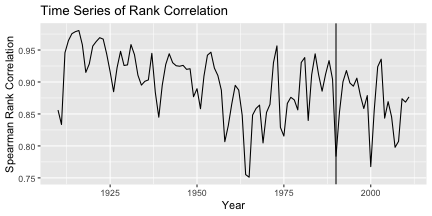
\includegraphics{Question1_files/figure-latex/Figure2-1} 

}

\caption{Caption Here \label{Figure2}}\label{fig:Figure2}
\end{figure}

The plot shows that there is a declining trend of the persistence of
popular names, which means that top names are usually shorter on the top
names list. Nonetheless the persistence still appears high enough that
we should not worry about tht for now.

\hypertarget{influence-of-other-variables}{%
\section{\texorpdfstring{Influence of other variables
\label{Meth}}{Influence of other variables }}\label{influence-of-other-variables}}

We know that pop culture can have an influence on names for new borns.
To be able to be the first to sell new nme personalized toys in the
future we will investigate if the actors who will play in popular movies
will have a strong influence on the names given to new borns.

We will start to invetigate the effect of movies on the names given to
newborns

\begin{verbatim}
## 
## Call:
## lm(formula = relative_change ~ in_movie, data = Popular_Names_with_following_year)
## 
## Residuals:
##    Min     1Q Median     3Q    Max 
## -31.57  -5.50  -1.37   1.86 392.47 
## 
## Coefficients:
##             Estimate Std. Error t value Pr(>|t|)
## (Intercept)   0.3382     1.4831   0.228    0.820
## in_movie      1.0357     1.4921   0.694    0.488
## 
## Residual standard error: 12.76 on 6195 degrees of freedom
## Multiple R-squared:  7.777e-05,  Adjusted R-squared:  -8.364e-05 
## F-statistic: 0.4818 on 1 and 6195 DF,  p-value: 0.4876
\end{verbatim}

\begin{figure}[H]

{\centering 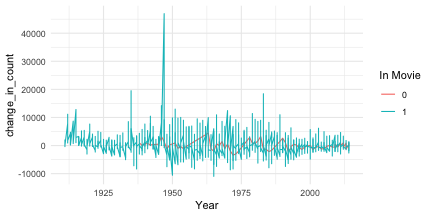
\includegraphics{Question1_files/figure-latex/Figure3-1} 

}

\caption{Caption Here \label{Figure3}}\label{fig:Figure3}
\end{figure}

\newpage

\bibliography{Tex/ref}





\end{document}
